\chapter{Establishing a Baseline}
\label{ch:baseline}

This chapter establishes a robust baseline for the IEEE 14-bus task. First, we tune a decentralized MLP-based MAPPO agent to achieve stable training and high survival rates. Second, we replace the flat MLP actor with a Graph Neural Network (GNN) encoder. 
\\
\\
This architectural shift is essential for generalizability: an MLP's input size is strictly tied to a specific grid size, preventing transferability. In contrast, a shared GNN encoder processes graphs of arbitrary sizes, theoretically enabling zero-shot transfer across different power grids. If a GNN encoder proves viable and competitive with the optimized MLP, it justifies investigating the optimal graph representation of the power grid, which is addressed in Chapters~\ref{ch:methods} and~\ref{ch:experiments}.

% \section{How to Read This Chapter}
% \label{sec:results-structure}

% This chapter is organized as a sequence of experiment blocks, and the later
% experimental chapters reuse the same pattern. Each block follows the same
% structure:

% \begin{enumerate}
%   \item \textbf{Question.} What uncertainty or design choice does this test
%   address?
%   \item \textbf{Baseline and change.} Which run is the control, and what is
%   changed in the comparison runs?
%   \item \textbf{Protocol.} Which data split, checkpoint, seeds, and metric are
%   used?
%   \item \textbf{Implementation detail.} Which algorithmic, architectural, or
%   mathematical change is being tested, when this is relevant?
%   \item \textbf{Evidence.} Which table and figure summarize the result?
%   \item \textbf{Interpretation.} What can be concluded, and what still needs to
%   be verified?
% \end{enumerate}

\section{Evaluation Protocol}
\label{sec:results-evaluation-protocol}

All experiments use an 80/20 train/test chronic split. The 80\% training split is used for policy updates, while the 20\% test split estimates generalization. Evaluation rollouts run periodically during training using 10 episodes per split. 
\\
\\
The primary performance metric is test episodic survival (expressed as a percentage), representing the fraction of evaluation episodes where the agent successfully prevents a blackout. Results are reported using seed-aggregated mean curves, with shaded regions indicating variability. Final evaluations report the performance of the checkpoint that achieved the highest test survival during training.

\section{Experiment Index}
\label{sec:results-experiment-index}

\begin{table}[H]
  \centering
  \small
  \caption{Current result blocks and their role in the thesis.}
  \label{tab:experiment-index}
  \setlength{\tabcolsep}{4pt}
  \begin{tabular}{L{0.2\textwidth}L{0.37\textwidth}L{0.36\textwidth}}
    \toprule
    Block & Main question & Primary evidence \\
    \midrule
    MLP baseline reruns & Which baseline training changes stabilize MAPPO? &
    Table~\ref{tab:a0-core-summary}, Figures~\ref{fig:rerun-a0-pairwise}
    and~\ref{fig:rerun-a0-all} \\
    Initial do-nothing bias & Does biasing initial exploration toward do-nothing help? &
    Table~\ref{tab:a0-bias-summary}, Figure~\ref{fig:rerun-a0-bias} \\
    GINE reruns & Do graph encoders improve survival over the optimized MLP baseline? &
    Tables~\ref{tab:gine-run-configurations} and~\ref{tab:gine-rerun-summary},
    Figure~\ref{fig:rerun-gine-best00}\\
    Heavy GINE & Does a larger GINE architecture help or overcomplicate
    optimization? & Table~\ref{tab:heavy-gine-configurations},
    Figure~\ref{fig:gine-best-search2} \\
    \bottomrule
  \end{tabular}
\end{table}

\section{IEEE 14-Bus Experiments}
\label{sec:bus14-results}

The initial PPO/MAPPO baseline from the MARL2Grid framework yielded unstable policies and low survival rates on the IEEE 14-bus topology-control task. The following experiments systematically test training and architectural modifications to establish a high-performing baseline.

\subsection{MLP Baseline}
\label{subsec:a0-core-reruns}

\paragraph{Question.}
Which changes are needed to obtain a stable MLP MAPPO baseline on the 14-bus
task?

\paragraph{Baseline and changes.}
We start from the MLP MAPPO baseline of the MARL2Grid framework and test several main
stabilization choices:

\begin{itemize}
  \item increasing actor and critic capacity from two hidden layers to three
  hidden layers;
  \item using reward normalization;
  \item changing the critic update so that the critic is updated once for the
  whole batch instead of once per agent;
  \item tuning of optimization hyperparameters to stabilize the training, as summarized in Table~\ref{tab:new-hyperparameters}.
\end{itemize}

\begin{table}[H]
  \centering
  \small
  \caption{New hyperparameters for MAPPO training.}
  \label{tab:new-hyperparameters}
  \begin{tabular}{lrr}
    \toprule
    Hyperparameter & New Value & Paper Baseline \\
    \midrule
    \textbf{ENVIRONMENT} & & \\
    n\_envs (number parallel environment) & 20 & 10 \\
    \midrule
    \textbf{PPO OPTIMIZATION} & & \\
    Total time step & 15,000,000 & 25,000,000 \\
    Actor learning rate & 1e-4 & 3e-5 \\
    Critic learning rate & 1e-4 & 3e-5 \\
    Gamma & 0.9 & 0.99 \\
    Update epochs & 10 & 80 \\
    Minibatches & 16 & 4 \\
    Maximum gradient norm & 1.0 & 10.0 \\
    \bottomrule
  \end{tabular}
\end{table}

\paragraph{Evidence.}
Table~\ref{tab:a0-core-summary} reports final and peak survival for the core
ablations. Figure~\ref{fig:rerun-a0-pairwise} shows each comparison against the
\texttt{Optimized MLP Baseline}, and Figure~\ref{fig:rerun-a0-all} overlays all
core MLP baseline curves.

\paragraph{Interpretation.}
The \texttt{Optimized MLP Baseline}, which combines three hidden layers, reward normalization, and an optimized critic update, achieves the best performance and convergence speed, yielding the highest and most stable final survival (\(\sim\)93\%). Removing or reducing any of these three elements, using a smaller architecture, disabling reward normalization, or reverting to a non-optimized critic update, results in a drop in either learning speed or final survival. The original unoptimized baseline fails entirely to learn a competitive policy. Because the \texttt{Optimized MLP Baseline} consistently outperforms the ablations, it is established as the standard reference for all subsequent comparisons.

\begin{table}[H]
  \centering
  \scriptsize
  \caption{MLP baseline run configurations. The reference run is
  \texttt{Optimized MLP Baseline}.}
  \label{tab:a0-run-configurations}
  \setlength{\tabcolsep}{3pt}
  \begin{tabular}{L{0.25\textwidth}L{0.13\textwidth}L{0.09\textwidth}L{0.11\textwidth}L{0.11\textwidth}L{0.20\textwidth}}
    \toprule
    Run family & Actor/critic hidden layers & Reward norm. & Initial action-0 prob. &
    Optimized critic update & Difference from \texttt{Optimized MLP Baseline} \\
    \midrule
    \texttt{Optimized MLP Baseline} & \(3\times256\) / \(3\times256\) &
    true & 0.0 & true & Reference baseline \\
    \texttt{Disable optimized critic update} & \(3\times256\) / \(3\times256\) &
    true & 0.0 & false & Disables optimized critic updates \\
    \texttt{Smaller MLP actor/critic} & \(2\times256\) / \(2\times256\) &
    true & 0.0 & true & Uses a smaller MLP actor and critic \\
    \texttt{Disable reward normalization} & \(3\times256\) / \(3\times256\) &
    false & 0.0 & true & Disables reward normalization \\
    \texttt{Old baseline (no val)} & \(3\times256\) / \(3\times256\) &
    true & 0.3 & false & Uses action-0 bias 0.3 and non-optimized critic updates \\
    \texttt{Initial Bias 50\%} & \(3\times256\) / \(3\times256\) &
    true & 0.5 & true & Uses action-0 bias 0.5 \\
    \texttt{Initial Bias 70\%} & \(3\times256\) / \(3\times256\) &
    true & 0.7 & true & Uses action-0 bias 0.7 \\
    \bottomrule
  \end{tabular}
\end{table}

\begin{figure}[H]
  \centering
  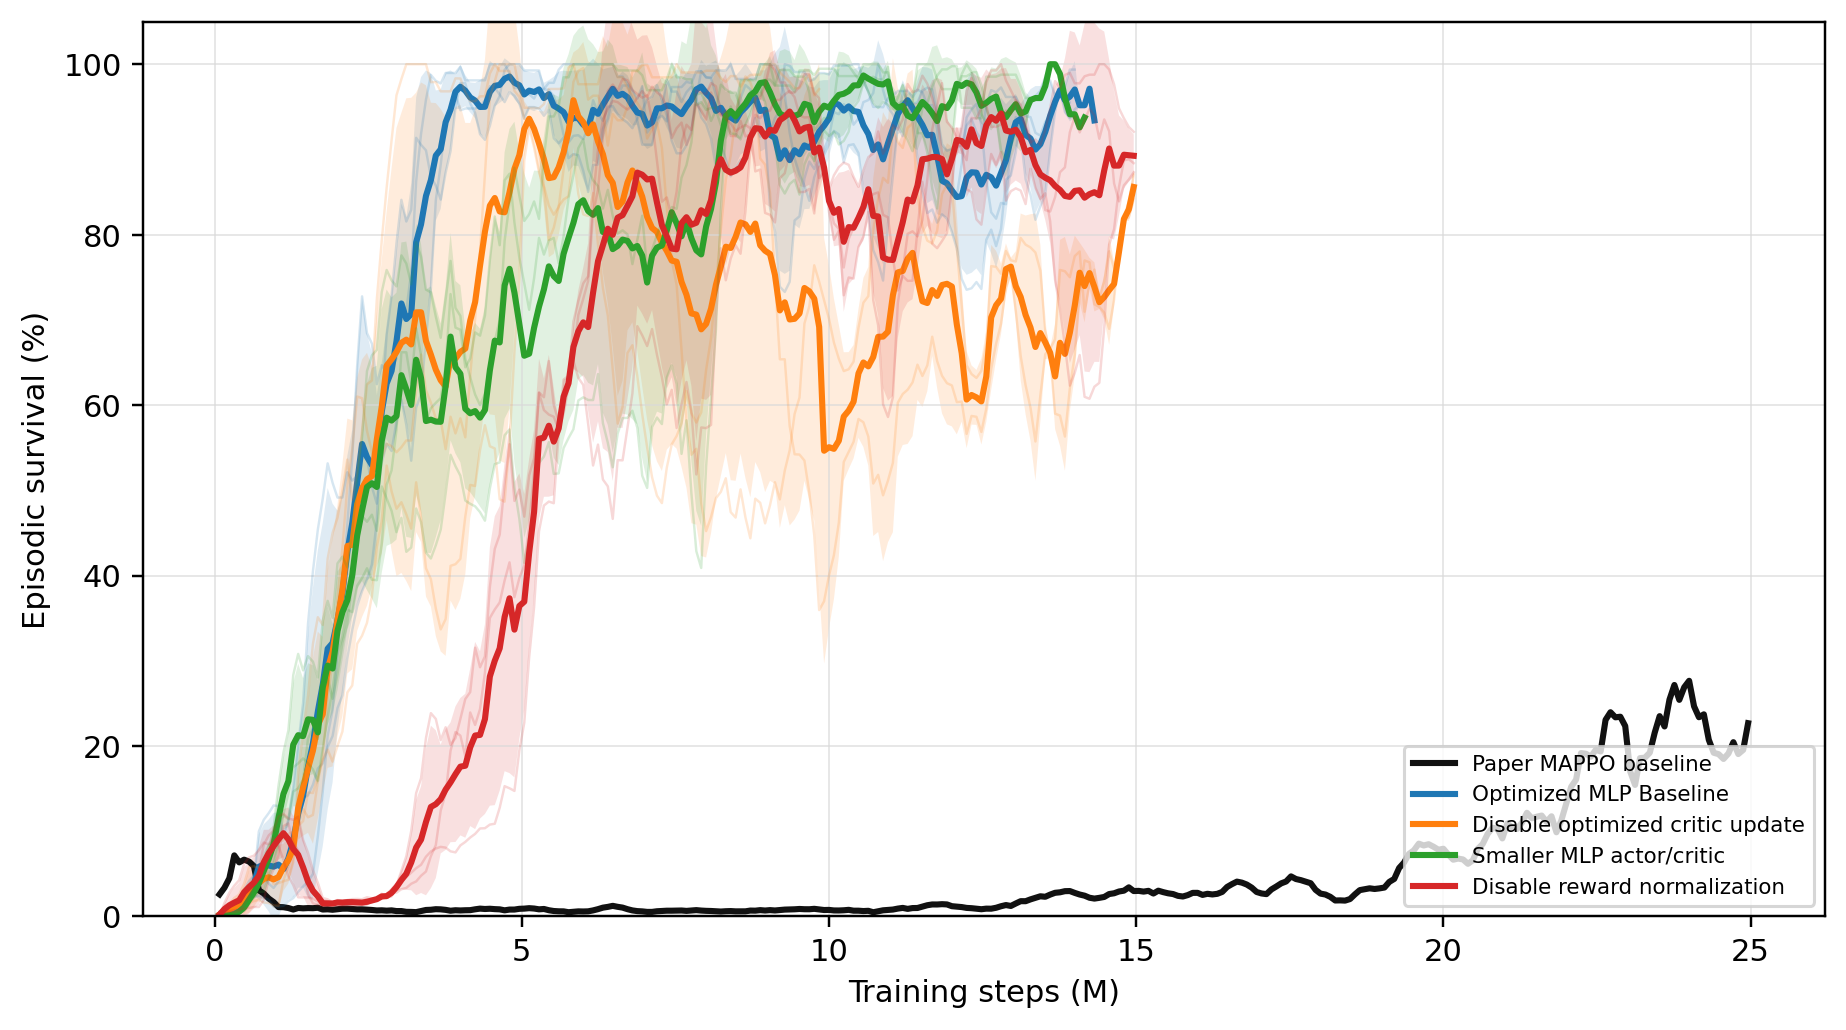
\includegraphics[width=\textwidth]{figures/rerun_a0_core_all_curves.png}
  \caption{All MLP baseline core rerun survival curves shown on one axis.}
  \label{fig:rerun-a0-all}
\end{figure}

\begin{figure}[H]
  \centering
  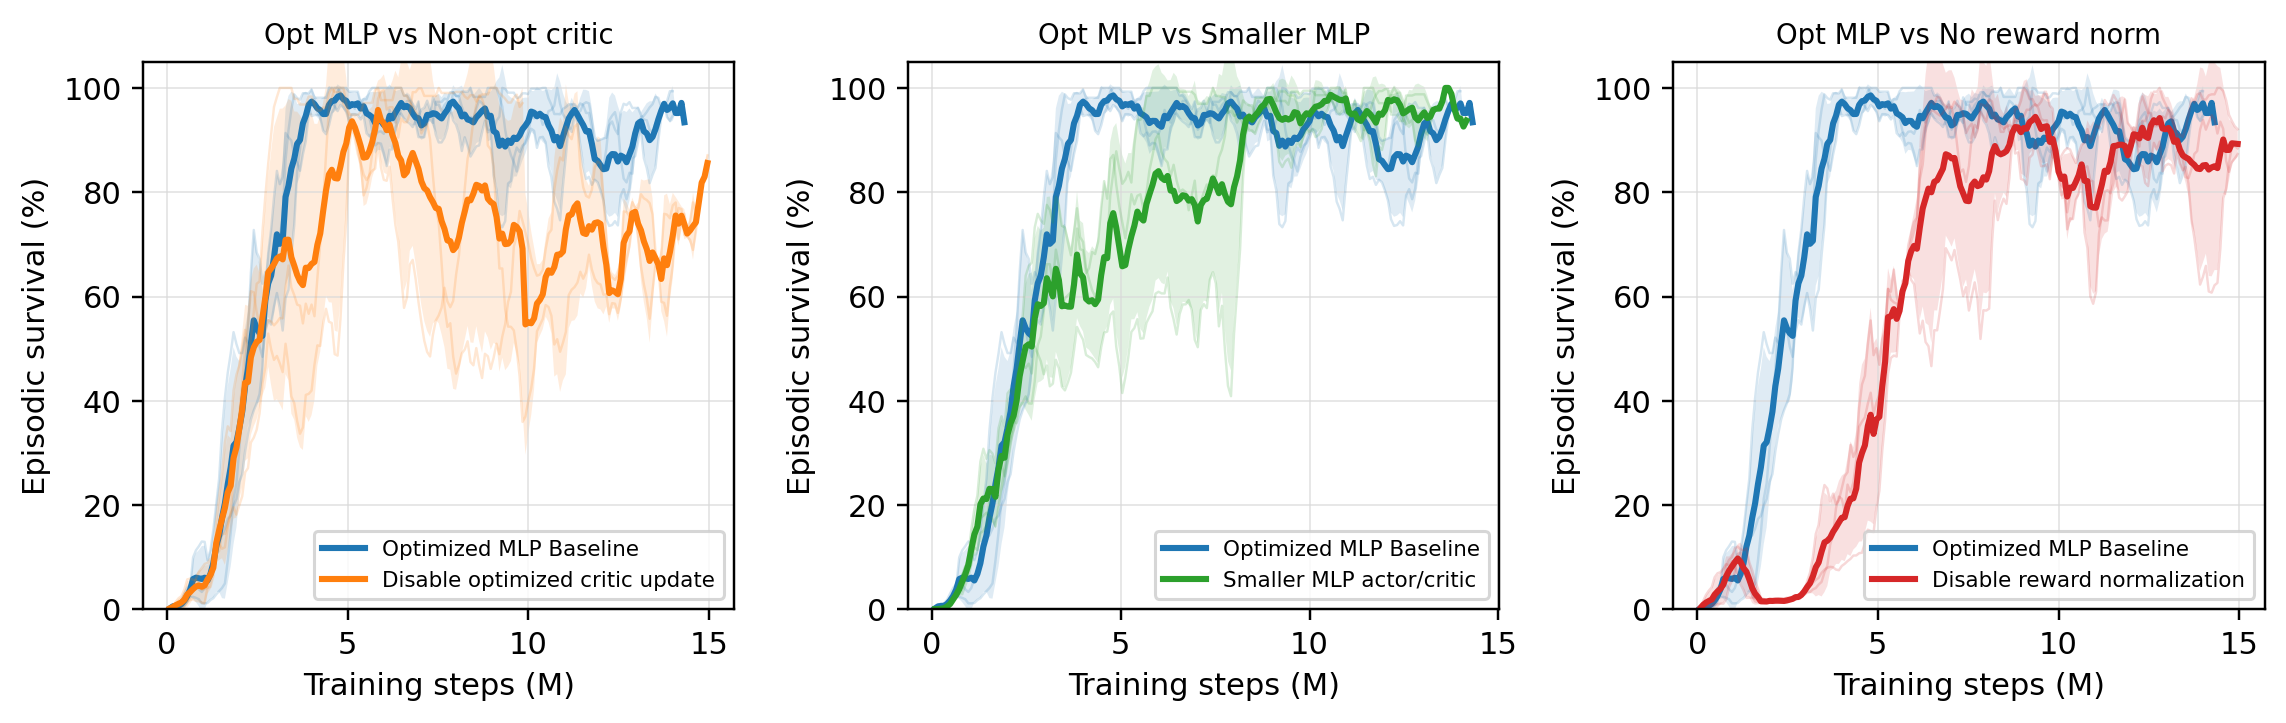
\includegraphics[width=\textwidth]{figures/rerun_a0_core_pairwise_comparisons.png}
  \caption{Pairwise MLP baseline rerun comparisons against the \texttt{Optimized MLP Baseline}.}
  \label{fig:rerun-a0-pairwise}
\end{figure}

\begin{table}[H]
  \centering
  \small
  \caption{MLP baseline core rerun survival summary.}
  \label{tab:a0-core-summary}
  \resizebox{\textwidth}{!}{%
  \begin{tabular}{llrr}
    \toprule
    Run & Intended change & Final survival (\%) & Peak survival (\%) \\
    \midrule
    \texttt{Optimized MLP Baseline} & Optimized MLP baseline & 93.4 & 98.6 \\
    \texttt{Disable optimized critic update} & Non-optimized critic update & 93.1 & 95.8 \\
    \texttt{Smaller MLP actor/critic} & Smaller MLP architecture & 93.7 & 100.0 \\
    \texttt{Disable reward normalization} & No reward normalization & 81.8 & 97.1 \\
    \bottomrule
  \end{tabular}
  }
\end{table}

% \hl{I need to run a full test eval on the best checkpoint of that MLP baseline}

\subsection{Initial Do-Nothing Bias}
\label{subsec:a0-bias-reruns}

\paragraph{Question.}
Does biasing the initial policy toward action 0, the do-nothing action, help or
hurt learning? In theory, a do-nothing bias makes sense because in reality, human operators most often do not operate the grid (i.e., they take no action) under normal conditions.

\paragraph{Baseline and changes.}
Our baseline uses no initial do-nothing bias in this rerun set. The bias
controls keep the same general protocol but change the initial probability mass
assigned to action 0.


\paragraph{Implementation detail.}
The bias is applied only at initialization: it changes the starting action
distribution before learning, without changing the reward, architecture, or PPO
objective. This is implemented by artificially increasing the initial pre-softmax logits for the do-nothing action, such that the policy initially selects this safe action with a higher probability before any learning updates occur. This makes the ablation a test of exploration bias rather than a test
of representational capacity.

\paragraph{Evidence.}
Table~\ref{tab:a0-bias-summary} and Figure~\ref{fig:rerun-a0-bias} compare the
zero-bias baseline with \texttt{Initial Bias 50\%} and
\texttt{Initial Bias 70\%}.

\paragraph{Interpretation.}
The effect of the action-0 bias is large and non-monotonic. The 0.5-bias curve
remains unstable and substantially below the zero-bias baseline, whereas the
0.7-bias curve eventually reaches the highest final survival in this comparison.
The current conclusion is that adding an initialization bias is generally hurtful or highly unstable for the models. Instead of aiding exploration, a strong initialization prior appears to restrict the agent's ability to reliably discover diverse beneficial actions and should be treated cautiously as a first-order ablation variable.

\begin{table}[H]
  \centering
  \small
  \caption{Initial do-nothing bias survival summary.}
  \label{tab:a0-bias-summary}
  \begin{tabular}{lrr}
    \toprule
    Run & Final survival (\%) & Peak survival (\%) \\
    \midrule
    \texttt{Optimized MLP Baseline} & 93.4 & 98.6 \\
    \texttt{Initial Bias 50\%} & 50.8 & 70.2 \\
    \texttt{Initial Bias 70\%} & 99.3 & 100.0 \\
    \bottomrule
  \end{tabular}
\end{table}

\begin{figure}[H]
  \centering
  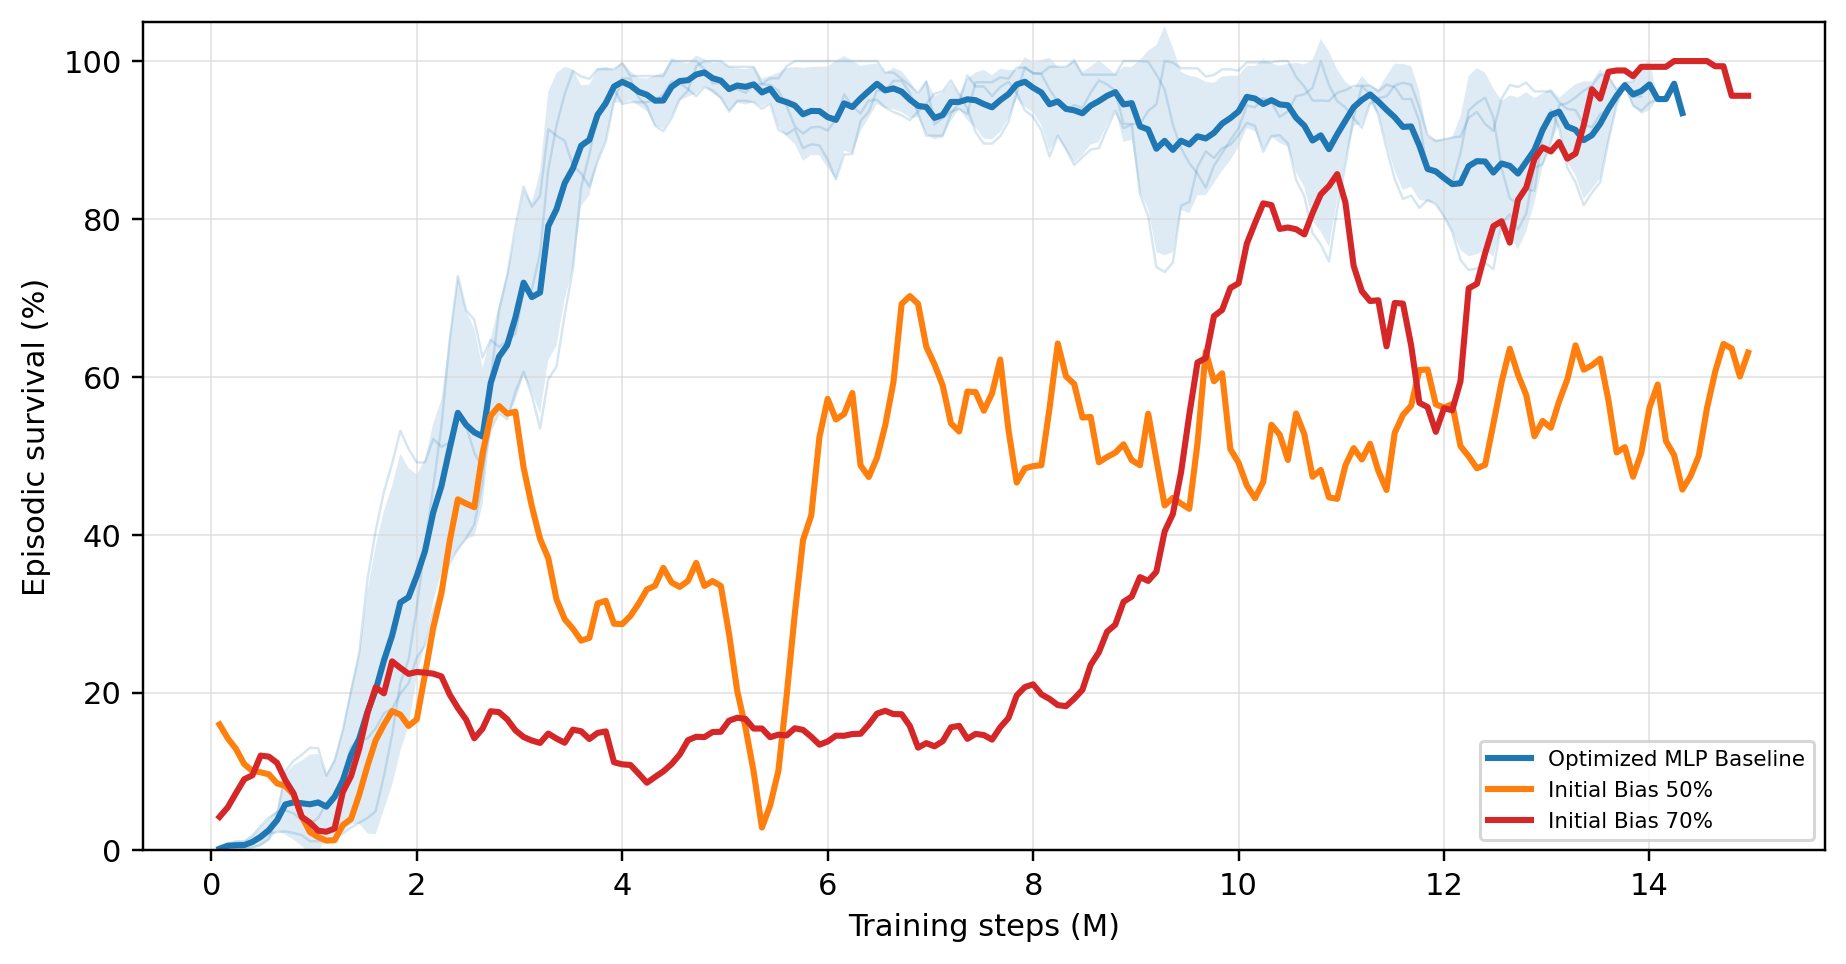
\includegraphics[width=\textwidth]{figures/rerun_a0_bias_comparison.png}
  \caption{Optimized MLP baseline compared with initial do-nothing bias controls
  \texttt{Initial Bias 50\%} and \texttt{Initial Bias 70\%}.}
  \label{fig:rerun-a0-bias}
\end{figure}

% \hl{I might need to run a full test eval of these runs}
% \hl{maybe i need to rerrun all these runs because they don't go/stop at 15M steps}

\subsection{Actor GNN Encoder Viability and Architecture}
\label{subsec:gnn-viability}

\paragraph{Question.}
Can a graph encoder perform as well as the MLP? This is a crucial question because if all agents share the same GNN encoder, the architecture becomes independent of the grid size and could maybe transfer to any grid topology. If each agent requires its own separate encoder or if the GNN cannot stabilize, this transferability is lost.

\paragraph{Baseline and changes.}
We conducted an exploratory study comparing several variations of the GINE architecture. We tested the encoder size (light vs. heavy GINE), actor sharing (shared vs. unshared encoder), the critic architecture (MLP vs. GNN), and the impact of the optimizations we established for the MLP baseline (optimized critic updates, reward normalization). 

\paragraph{Protocol.}
All GINE runs use \texttt{gnn\_type = gine}, \(15{,}000{,}000\) total timesteps, evaluation every \(80{,}000\) timesteps, \(2{,}000\) rollout steps, deterministic evaluation, and the same 80/20 chronic split used by the MLP experiments. We use GINE because it naturally incorporates edge features and has been shown to be powerful at distinguishing graph topologies \cite{xu2018how}. The complete graph-actor pipeline is described in Appendix~\ref{app:gine-architecture}, and Appendix~\ref{app:experiment-configurations} details the exhaustive parameter configurations used for these ablations in Tables~\ref{tab:gine-run-configurations} and~\ref{tab:heavy-gine-configurations}.

\paragraph{Evidence.}
Table~\ref{tab:gine-rerun-summary} and Figure~\ref{fig:rerun-gine-best00} compare the core architectural improvements against the \texttt{MLP Baseline}. Figure~\ref{fig:gine-best-search2} provides a broader search, showing how the baseline reacts to individual isolated changes.

\begin{table}[H]
  \centering
  \small
  \caption{GINE rerun survival summary.}
  \label{tab:gine-rerun-summary}
  \resizebox{\textwidth}{!}{%
  \begin{tabular}{llrr}
    \toprule
    Run & Intended change & Final survival (\%) & Peak survival (\%) \\
    \midrule
    \texttt{Heavy GINE Baseline} & Historical GINE baseline & 59.2 & 93.9 \\
    \texttt{Light GINE (Concat, MLP Critic)} & Light GINE with MLP critic & 78.9 & 90.4 \\
    \texttt{No Bias, Opt Critic} & Optimized critic and bias 0.0 & 82.5 & 85.7 \\
    \texttt{Optimized Light GINE} & Light optimized GINE with MLP critic & 95.7 & 97.4 \\
    \bottomrule
  \end{tabular}
  }
\end{table}

\begin{figure}[H]
  \centering
  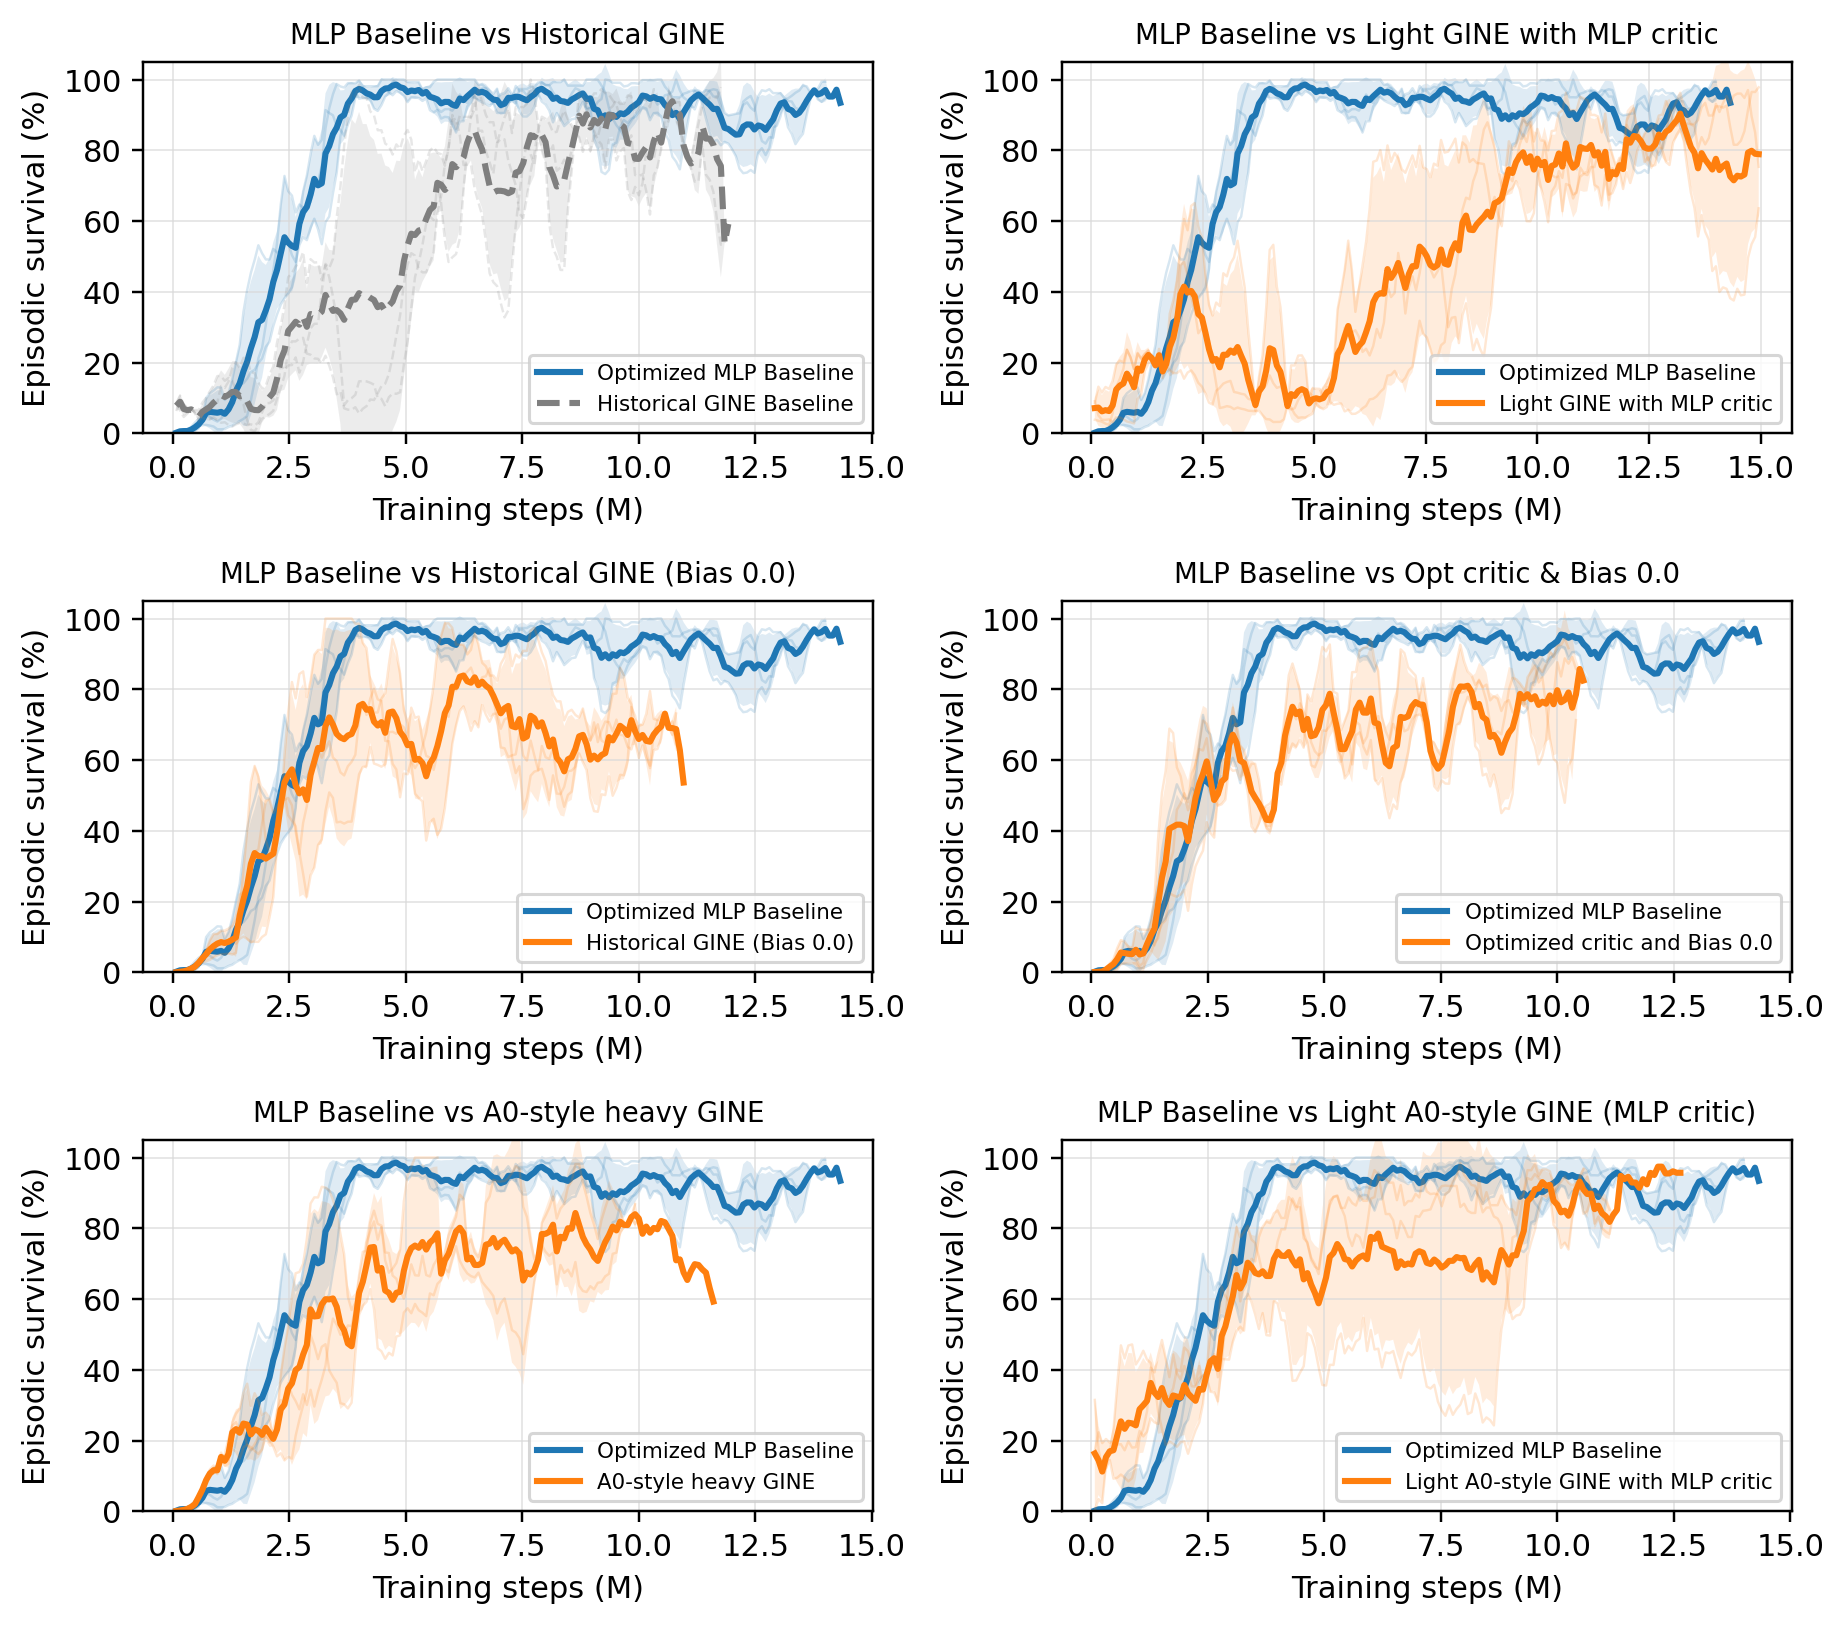
\includegraphics[width=\textwidth]{figures/rerun_gine_best00_vs_best10_14.png}
  \caption{Seed-aggregated test episodic survival comparing the \texttt{MLP Baseline} against high-performing GINE architectural modifications.}
  \label{fig:rerun-gine-best00}
\end{figure}

\begin{figure}[p]
  \centering
  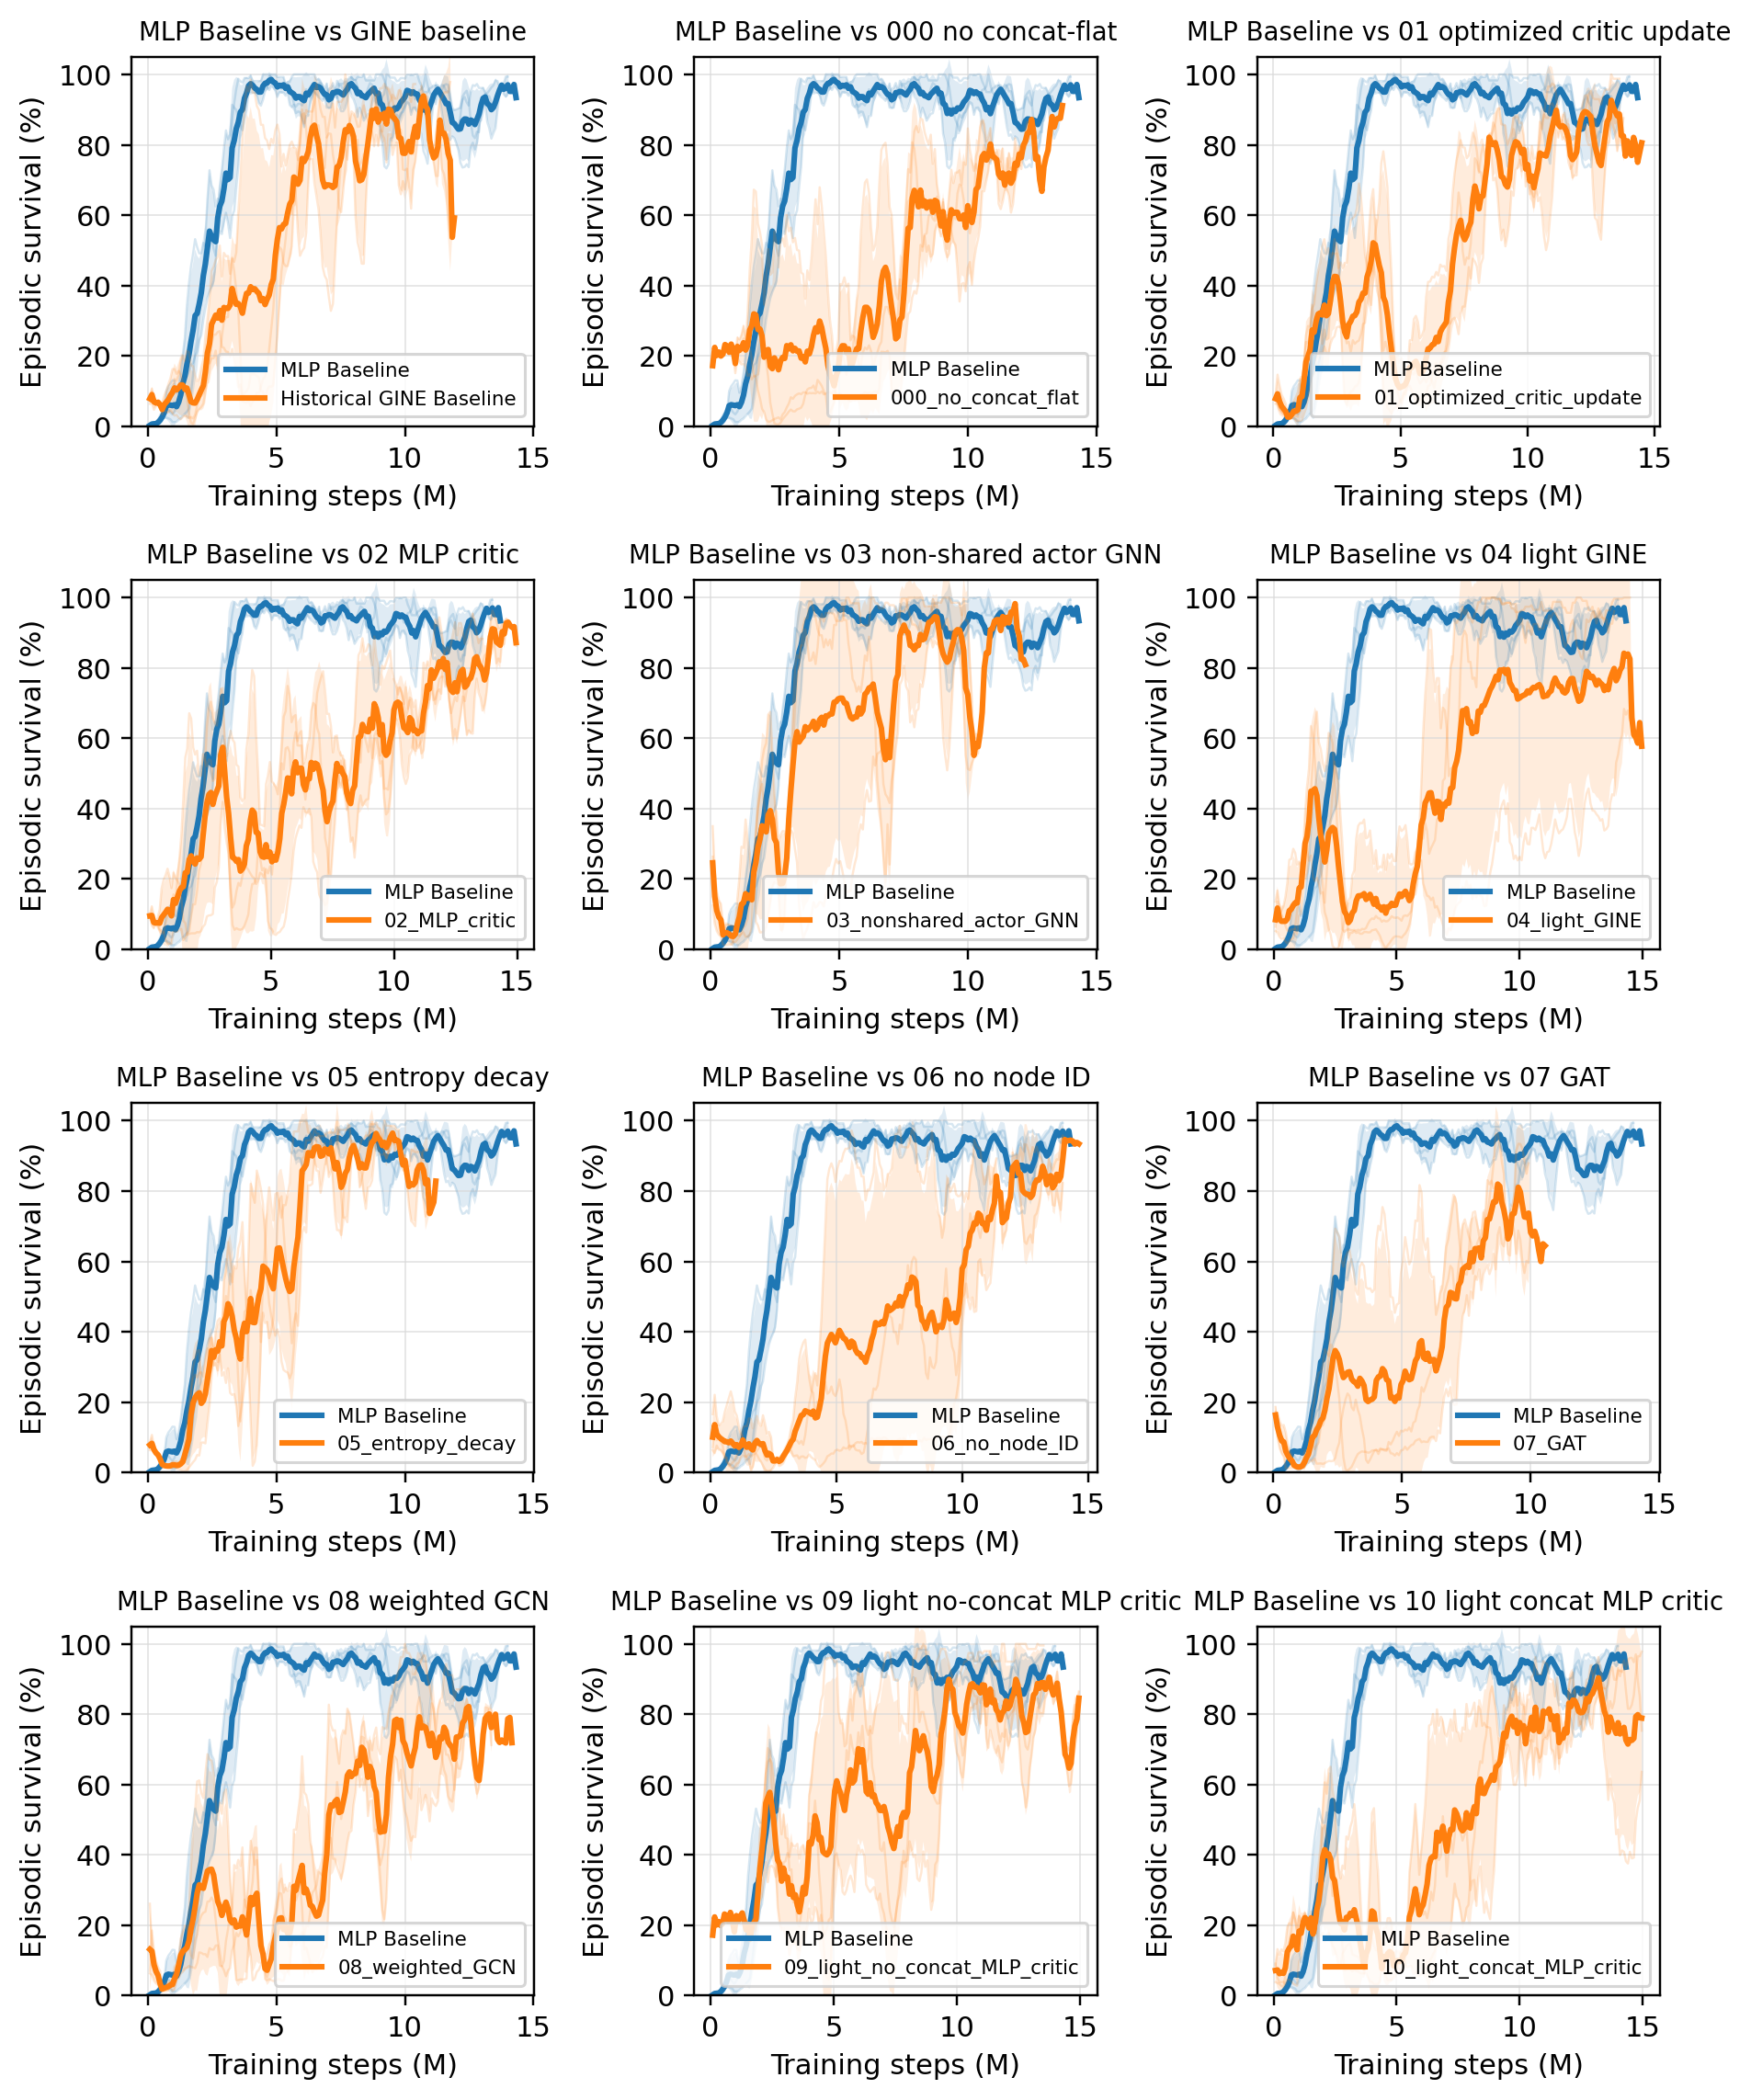
\includegraphics[width=\textwidth,height=0.9\textheight,keepaspectratio]{figures/gine_best_search2_baseline_comparisons.png}
  \caption{GINE survival comparisons. Each subplot compares the \texttt{MLP Baseline} against a specific GINE variant from \texttt{configs/gine\_s0\_s1\_s2}. All runs are modifications of a baseline GINE model; full hyperparameters and architectural details are provided in Appendix~\ref{app:gine-architecture} and Appendix~\ref{app:experiment-configurations}.}
  \label{fig:gine-best-search2}
\end{figure}

\paragraph{Interpretation.}
The results from the broad search provide several critical takeaways regarding the GNN architecture:
\begin{itemize}
  \item \textbf{Shared Encoder Viability:} As shown in Figure~\ref{fig:gine-best-search2}, the \texttt{Unshared Actor} variant does not outperform the other runs. This proves that a single shared GNN encoder for all agents is achievable and does not bottleneck performance, which is exactly what is needed for transferability.
  \item \textbf{Critic Architecture:} Attempting to use a GNN for the centralized critic proved unstable and degraded performance. The \texttt{MLP Critic} variants were significantly more stable. The best performance is clearly achieved by pairing the shared GNN actor with a standard MLP critic.
  \item \textbf{Optimization Synergies:} The GNN architecture is heavily dependent on the same optimizations that stabilized our MLP baseline. Specifically, optimized critic updates, reward normalization, and removing the initial do-nothing bias (bias 0.0) were crucial for getting the GNN to learn reliably.
\end{itemize}

\noindent The strongest overall result is the \texttt{Optimized Light GINE}, which combines the shared light GINE actor, the MLP critic, and all the baseline optimizations to reach \(95.7\%\) final survival. This validates that a GNN encoder is highly competitive on the 14-bus task.
\\
\\

\begin{tcolorbox}[colframe=red!75!black, colback=red!5!white, title=Chapter Summary]
\textbf{Objective:} Establish a stable, high-performing MAPPO baseline and validate the viability of a GNN encoder.

\textbf{Findings:}
\begin{itemize}
    \item \textbf{MLP Optimization:} Tuning hyperparameters, enabling reward normalization, and optimizing critic updates increased the flat MLP baseline survival to \(\sim\)93\%.
    \item \textbf{GNN Viability:} Replacing the MLP actor with a GNN (GINE) is highly competitive. Combined with our baseline optimizations, the \texttt{Optimized Light GINE} achieved \(95.7\%\) survival.
    \item \textbf{Transferability (Shared Actor):} A shared GNN encoder for all agents performs optimally. This is critical: because the encoder processes subgraphs of consistent dimensions regardless of the global grid size, a shared GNN actor theoretically enables zero-shot transferability to larger grids.
    \item \textbf{Critic Architecture:} The centralized critic observes the entire global graph, inherently tying it to the training grid's specific size. Consequently, a GNN critic offers no transferability benefits and was empirically found to induce training instability. We therefore retain a standard MLP critic.
\end{itemize}

\textbf{Conclusion:} We have proven that a shared GNN encoder is viable, providing us with an architecture that is structurally transferable and performs excellently on the IEEE 14-bus grid. However, while the architecture allows for transferability in theory, we do not yet know how it will perform in practice when transferred to a different grid. To address this, the next logical step is to explore the optimal ways to represent and process the power grid as a graph, identify the best representation, and attempt transferring it to a larger environment. Chapter~\ref{ch:methods} defines these representational spaces, and Chapter~\ref{ch:experiments} evaluates them.
\end{tcolorbox}


